\setchapterstyle{kao}
\chapter{Deep Learning}
\labch{deeplearning}

Differentiable programming \sidecite{blondel_2024, scardapane_2024} represents a
paradigm where the algorithms and functions within a program are designed to be
differentiable. This capability allows for the automatic adjustment of
parameters based on the data they process, facilitating the application of
gradient-based optimization methods. Essentially, differentiable programming
turns traditional programming constructs into learnable and adaptable entities,
enabling the development of systems that can efficiently learn from vast
datasets and complex environments.

The roots of differentiable programming can be traced back to the early
applications of calculus in computational tasks, where differentiation and
integration were used to solve physics-based and engineering problems. With the
advent of digital computing, these methods were translated into algorithms that
could be executed on machines. Over time, as the need for more sophisticated
data analysis and modeling grew, especially with the burgeoning field of
artificial intelligence, the methods evolved into what we now recognize as
differentiable programming.

The concept gained significant traction in the late 20th and early 21st
centuries, driven by the growth of machine learning and particularly the
resurgence of neural networks. The development of automatic differentiation
technologies marked a pivotal advancement, making it practical to implement and
train complex models that require the efficient calculation of derivatives. By
blurring the lines between traditional programming and machine learning,
differentiable programming has created a new toolbox for problem solving, one
that is inherently flexible, powerful, and suited to a range of applications
that extend far beyond its origins. This blend of flexibility and power forms
the bedrock upon which modern machine learning, especially deep
learning, builds to achieve remarkable feats across
various domains.

Deep learning \sidecite{lecun_2015, goodfellow_2016} stands as a prominent
example of differentiable programming in action, illustrating the power and
versatility of this computational paradigm. At its core, deep learning involves
systems that are intricately designed to learn from data by approximating
functions that map inputs to desired outputs. These mappings are not fixed;
instead, they are dynamically refined through the model's learnable parameters,
which fundamentally determine the output of the function.
For example, \refeq{2_1} illustrates a series of parameterized maps, each with
one and two parameters respectively ($\theta_0$ and $\theta_0, \theta_1$
respectively).
\begin{equation}
\labeq{2_1}
f(x; \theta)=\theta_0 x \quad f(x; \theta) = \theta_0 x + \theta_1 x
\end{equation}
The optimization of these parameters is where the principles of differentiable
programming become essential. Deep learning models adjust their parameters
\sidenote{Namely weights and biases.} based on the input data they receive and
the feedback (loss\sidenote{Which measure how far the model's predictions
deviate from the actual values.}) related to the accuracy of their outputs.
This adjustment is achieved through gradient-based optimization methods, a
process central to the training and effectiveness of deep learning systems.
From this discussion it's possible to clearly delineate the main components
essential to deep learning:
\begin{itemize}
    \item \textbf{Model}: a function $f(x; \theta)$ parametrized by $\theta$.
    \item \textbf{Dataset}: a supervised dataset $\mathcal{D}_n$ of size $n$ is a
    set of $n$ pairs $\mathcal{D}_n = \{(x_i, y_i)\}^n_{i=1}$, where each $(x_i, y_i)$
    is an example of an input-output relationship that the model must approximate.
    \item \textbf{Loss}: a \emph{differentiable} function $L(y, \hat{y})$ that
    given a desired target $y$ and the predicted value $\hat{y}=f(x)$,
    qualifies the discrepancy between the model's prediction and the
    actual value $y$.
    \item \textbf{Optimization method}: an algorithm that adjusts the model’s
    parameters $\theta$ to minimize the average loss across the entire
    dataset.
\end{itemize}
As previously discussed, the essence of deep learning involves developing
models that approximate the relationship between inputs and outputs using only
a limited subset of data points (the dataset). These models learn from this
dataset by minimizing a loss function, which quantifies the extent of incorrect
predictions. Building on the definitions provided earlier, this learning
process can be structured as an optimization problem.
\begin{equation}
\labeq{2_2}
\theta^* = \arg \min_{\theta} \frac{1}{n} \sum_{i=1}^n L(y_i, f(x_i; \theta))
\end{equation}
\refeq{2_2} formalizes the objective of the optimization problem in deep
learning, which involves identifying a set of parameters $\theta$ that minimizes
the average loss across the entire dataset. This method approximates the
expected loss across the general distribution, ensuring that the model $f(x;
\theta^*)$ is optimally accurate in mapping inputs to their correct outputs by
closely estimating the true risk\sidenote{The optimization problem adheres to
the empirical risk minimization (ERM) principle, which leverages the law of
large numbers to approximate how well a predictive model will perform in
practice. Since the true distribution of data is unknown, ERM focuses on
minimizing the observed loss on a specific dataset, referred to as the
"empirical risk."} with the available data.

\section{Gradient Based Optimization}
To solve the optimization problem formalized in ~\refeq{2_2}, gradient-based
optimization methods are predominantly employed, especially in deep learning.
These methods are highly effective due to their ability to manage the
complexities and extensive scale of neural network training, and are
particularly well-suited for navigating the intricate loss landscapes that arise
from the non-linear activation functions typical of deep networks. Unlike
simpler models, deep learning architectures often feature complex, non-convex
loss functions that lack analytical solutions, making gradient-based approaches
essential for finding approximate solutions. A significant advantage of
gradient-based methods is their flexibility and generality, which allows them to
be applied across a wide range of problem settings and architectures without
specific tailoring to the task. This versatility is enhanced by their efficiency
in high-dimensional spaces, a common feature in neural networks that often
include millions of parameters.
Gradient-based optimization methods rely on calculating the
\emph{gradient}\sidenote{A gradient is the generalization of the concept of a
derivative to functions of multiple variables. While a derivative gives the rate
of change of a function with respect to one variable, the gradient extends this
idea to vector fields. The gradient is then a vector that points to the
direction of the steepest ascent of a function in any specific point.}
$\nabla_\theta L$ of the loss function $L$ with respect to the model's
parameters $\theta$. The optimization method then iteratively adjusts the
parameters in the opposite direction of the gradient.
\begin{equation}
    \labeq{2_3}
    \theta_t = \theta_{t-1} - \gamma \cdot \nabla_{\theta} \left ( \frac{1}{n} \sum^n_{i=1} L(y_i, f(x_i; \theta_{t-1})) \right )
\end{equation}
\refeq{2_3} shows the update rule applied at each iteration, where the
parameters for the next iteration, $\theta_t$, are derived by reducing the
current parameters $\theta_{t-1}$ by a small fraction of the gradient of the
expected loss across the dataset. This fraction is governed by $\gamma$,
commonly referred to as the \emph{learning rate}, which directly influences the
magnitude of each step in the iterative process. The update rule is typically
applied over a number of iterations referred to as \emph{epochs}, which
correspond to the number of times the entire dataset is processed.

Geometrically, this update rule can be visualized as a method for navigating
the multidimensional landscape defined by the loss function. Here, $\theta$
represents a point in this landscape, and the gradient of the loss function at
this point indicates the direction of steepest ascent. By moving in the
opposite direction, which is the negative gradient, the update rule effectively
seeks the path of steepest descent, thereby taking steps that effectively
minimize the loss.

\begin{marginfigure}
  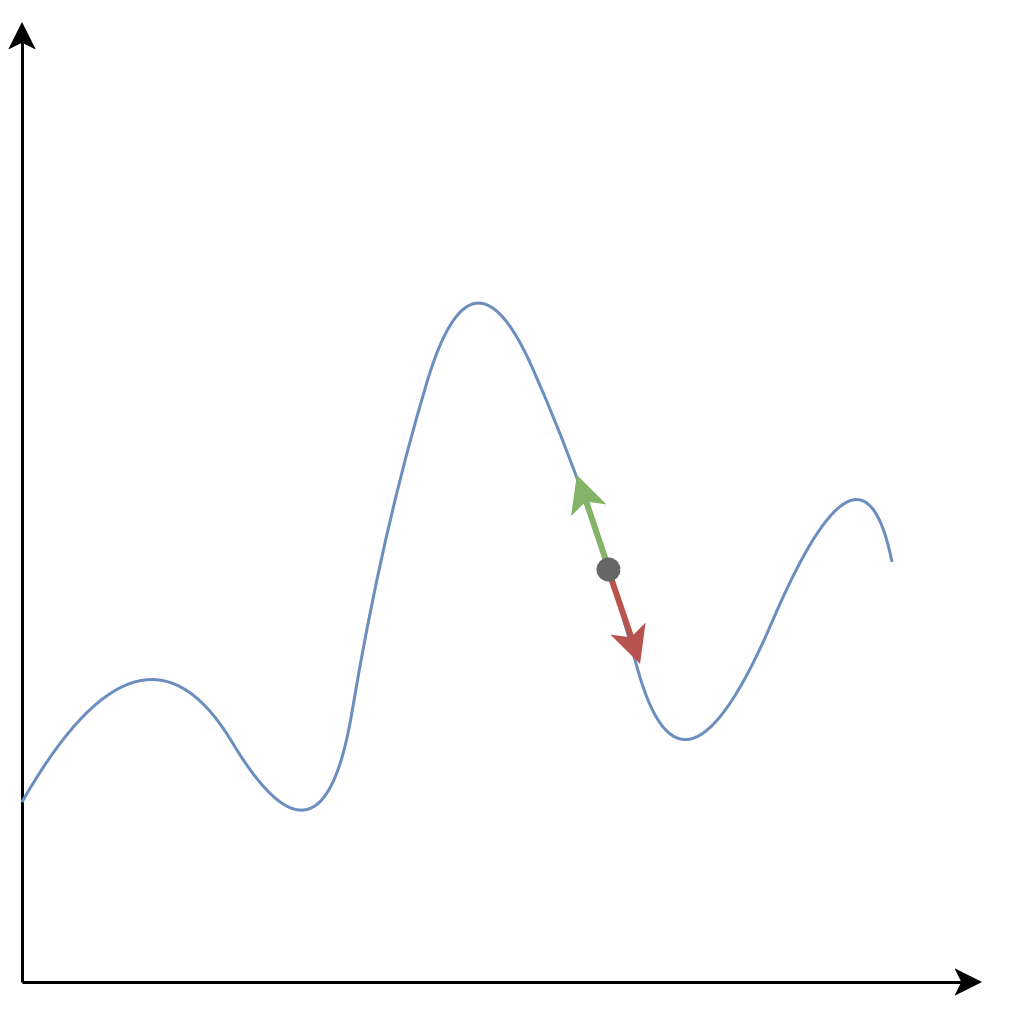
\includegraphics{2_1_points_gradients}
  \labfig{2_1}
  \caption[Gradient and Loss]{The gradient (green arrow) of a function evaluated
  in a specific point (gray) indicates the direction of the steepest ascent from
  that point. Conversely, the opposite of the gradient (red arrow) indicates the
  direction of the steepest descent. }
\end{marginfigure}

This method of using gradients to optimize function parameters, highlights a
crucial aspect of differentiable programming: every component of the
computational model, especially those that impact learning and prediction,
needs to be differentiable in terms of their parameters. Moreover, the
effectiveness of the optimization hinges directly on the efficiency with which
gradients are computed. Consequently, it is essential to have a robust method
for this computation to ensure the optimization process is both accurate and
efficient.

\subsection{Automatic Differentiation}
Automatic differentiation (AD) is a computational technique that efficiently
and accurately computes derivatives of functions. Unlike symbolic
differentiation, which manipulates mathematical symbols to produce derivative
formulas, or numerical differentiation, which approximates derivatives using
finite differences, AD operates directly on numerical values and applies the
chain rule to compute derivatives of composed functions. To fully understand
the utility and mechanics of Automatic Differentiation and the specific
challenges it addresses, it is crucial to first explore the two prevalent
methods used to compute derivatives on a computer. The first is \emph{symbolic
differentiation}, which involves manipulating the mathematical symbols of the
original expression through a set of transformation rules\sidenote{For
instance, the derivative $\frac{\partial \sin(x)}{\partial x}$ is $\cos(x)$.}.
By systematically applying these rules, one can derive an expression that can
be used to compute the gradient at any point, provided that the derivative is
continuous. Symbolic differentiation is considered stable in that it does not
introduce computational error. However, it is often challenging to implement
and can be computationally inefficient compared to other methods, particularly
as the function expressions become more complex and the expressions for their
derivatives increase drastically in the number of terms. This exponential
growth in complexity can significantly hinder performance and scalability.
The second approach to computing derivatives, known as \emph{numerical
differentiation} or the \emph{finite difference} method, utilizes the
conventional definition to calculate the derivative at
a specific point. \refeq{2_4} shows the standard formula for divided
differences, which calculates the slope of the secant line through the points
$(x,f(x))$ and $(x+h,f(x+h))$. By selecting an infinitesimally small value for
$h$, it is possible to achieve an increasingly accurate approximation of the
true derivative.
\begin{equation}
    \labeq{2_4}
    f'(x) = \lim_{h \to 0} \frac{f(x + h) - f(x)}{h}
\end{equation}
While generally being more computationally efficient than the former (as it
does not require the precomputation of the derivative expression), a
significant drawback of this approach is its numerical stability; it can
introduce round-off errors during the discretization process, particularly when
computing derivatives of orders higher than the first. This susceptibility to
errors stems from the finite precision with which computers represent numbers,
which can lead to inaccuracies in the calculated derivatives, especially for
small differences in function values.
\marginnote{Generally speaking, numerical differentiation is particularly
useful when the exact analytical derivative is difficult to obtain, as it
allows for the practical estimation of derivatives using straightforward
numerical computations.}

Both classical methods of differentiation, symbolic and numerical, have their
advantages and disadvantages. However, their primary drawback lies in the slow
computation of partial derivatives of a function with respect to multiple
inputs, which is essential for gradient-based optimization
algorithms\sidenote{Especially in deep learning, where the gradient with
respect to million of parameters must be computed at each iteration of the
learning process.}.
Automatic differentiation effectively resolves all these issues by providing a
more efficient and rapid means to calculate these derivatives, thereby
enhancing the performance of algorithms that rely heavily on gradient
calculations.

Automatic differentiation capitalizes on the principle that all functions,
regardless of their complexity, are ultimately reducible to a sequence of
elementary arithmetic operations (such as addition, subtraction, multiplication,
and division) and elementary functions (like exp, log, sin, and cos). The key
idea of AD involves breaking down computations into elementary steps that create
an \emph{evaluation trace} \sidecite{griewank_derivatives_2008}. Each step’s
derivative is then integrated using the chain rule. Thanks to the utilization of
evaluation traces, AD is capable of differentiating not only through
calculations in closed form but also through control flow statements commonly
found in programming. Regardless of the specific computational pathway executed,
the numerical operations will generate an evaluation trace that can be employed
for AD.
An evaluation trace can be seen as the series of steps that are needed to reach
the final result. Consider, for example, the function $f: \mathbb{R}^n \to
\mathbb{R}^m$ (where $n=2$ and $m=1$) whose expression is provided
in~\refeq{2_5}.
\begin{equation}
\labeq{2_5}
    y=\left[\sin \left(\frac{x_{1}}{x_{2}}\right)+\frac{x_{1}}{x_{2}}-\exp
    \left(x_{2}\right)\right] \left[\frac{x_{1}}{x_{2}}-\exp
    \left(x_{2}\right)\right]
\end{equation}
Using the following notation:
\begin{itemize}
    \item $v_{i-n} = x_i, i = 1, \dots, n$ are the input variables.
    \item $v_{i}, i=1, \dots, l$ are the intermediate variables.
    \item $y_{m-i} = v_{l-i}, i=(m-1), \dots, 0$ are the output variables.
\end{itemize}
\begin{margintable}[*-12] %[ht]
    \caption[Evaluation Trace]{Evaluation trace of \refeq{2_5}.}
    \labtab{2_1}
    \centering
    \resizebox{\textwidth}{!}{
    \begin{tabular}{ c c c }
      \toprule
      Variable & Expression & Value \\
      \midrule
        $v_{-1}$ & $x_1$ & $1.5$ \\
        $v_0$ & $x_2$ & $0.5$ \\
        $v_1$ & $v_{-1}/v_0$ & $3.0$ \\
        $v_2$ & $sin(v_1)$ & $0.141$ \\
        $v_3$ & $exp(v_0)$ & $1.648$ \\
        $v_4$ & $v_1 - v_2$ & $1.351$ \\
        $v_5$ & $v_2 + v_4$ & $1.492$ \\
        $v_6$ & $v_5 \cdot v_4$ & $2.016$ \\
      \bottomrule
    \end{tabular}
    }
\end{margintable}
The expression shown in \refeq{2_5} can be decomposed into simpler components as
shown in~\refeq{2_6}. By assigning values to each input, $x_1, x_2$, and
sequentially evaluating each sub-expression, the final value of $y$ can be
obtained\sidenote{This procedure corresponds to executing the differentiable
program $f$, a process often referred to in deep learning as the \emph{forward
pass}. This term underscores the transformation of the input signal through
intermediate steps until the output is reached}.
\begin{equation}
    \labeq{2_6}
    \begin{split}
        v_{-1} &= x_1\\
        v_0 &= x_2\\
        v_1 &= v_{-1} / v_0\\
        v_2 &= sin(v_1)\\
        v_3 &= exp(v_0)\\
        v_4 &= v_1 - v_3\\
        v_5 &= v_2 + v_4\\
        v_6 &= v_5 \cdot v_4\\
    \end{split}
\end{equation}
For example, a possible run with $x_1=1.5$ and $x_2=0.5$ would lead to the
evaluation trace depicted in \reftab{2_1}. This evaluation trace is also
called \emph{Wengert List} \sidecite{wengert_1964}.
A logical progression in determining the derivative of $y$ with respect to its
inputs involves following the evaluation trace and computing the derivatives
sequentially for each intermediate variable. This approach forms the basis of
the \emph{forward mode} of the automatic differentiation algorithm.
\begin{figure}
  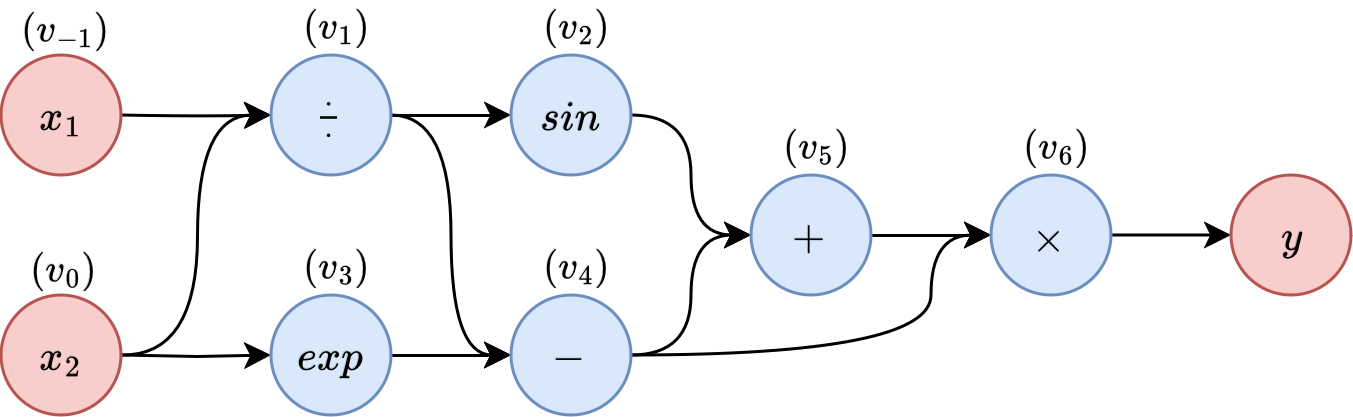
\includegraphics{2_2_computational_graph}
  \caption[Computational Graph]{\refeq{2_6} can also be represented
    graphically as a Directed Acyclic Graph (DAG). In this representation, blue
    nodes symbolize the intermediate operations, red nodes denote the
    input/output nodes, and the edges depict the algebraic relationships
    between these nodes.}
  \labfig{2_2}
\end{figure}
\subsubsection{Forward Mode}
Suppose the objective is to compute the derivative $\frac{\partial y}{\partial
t}$ with respect to an arbitrary input variable $t$. The chain rule
(\refeq{2_7}), offers a straightforward method for accomplishing this.
\begin{equation}
    \labeq{2_7}
    \der{u}{t} = \sum_i \left( \der{u}{v_i}\der{v_i}{t}\right)
\end{equation}\marginnote{\refeq{2_7} illustrates the application
of the chain rule in computing the gradient of $u$ with respect to any
intermediate variable $t$. The computation involves summing the products of
each partial derivative of $u$ with respect to its intermediate variables $v_i$
and the gradient of each intermediate variable $v_i$ with respect to the input
$t$.} The forward method of automatic differentiation involves calculating the
derivative $\dot{v}_i = \der{v_i}{t}$ for each intermediate variable
$v_i$. According to the chain rule (\refeqshort{2_7}), the derivative of each
variable $v_i$ is dependent on the values preceding it, allowing gradients to
be accumulated throughout the forward pass. This process is therefore aptly
named the \emph{forward accumulation mode}. To illustrate the dependency chain
integral to the process of forward accumulation,~\refeq{2_8}
demonstrates the computation of the derivative $\dot{v}_1$, emphasizing that
the current derivative value ($\dot{v}_1$) is contingent upon both the values
and derivatives of preceding variables ($v_0, v_{-1}$).
\begin{equation}
    \labeq{2_8}
    \begin{split}
        \dot{v}_1 &= \frac{\partial v_1}{\partial t}\\
        &= \frac{\partial v_1}{\partial v_{-1}}\frac{\partial v_{-1}}{\partial
        v_{t}} + \frac{\partial v_1}{\partial v_0}\frac{\partial
        v_0}{\partial v_t}\\
        &= \frac{\partial v_1}{\partial v_{-1}}\dot{v}_{-1} + \frac{\partial
        v_1}{\partial v_0}\dot{v}_0\\
        &= \frac{1}{v_0} \dot{v}_{-1} + \dot{v}_0 \left(-\frac{v_{-1}}{v_0^2}\right)
    \end{split}
\end{equation} By applying the same rule to each variable $v_i$, it is possible
to derive the formulas to compute the gradient of each intermediate variable of
the computation, as demonstrated in~\refeq{2_9}.
\begin{equation}
    \labeq{2_9}
    \begin{split}
        \dot{v}_{-1} &= \der{x_1}{t}\\
        \dot{v}_0 &= \der{x_2}{t}\\
        \dot{v}_1 &= \frac{1}{v_0}\dot{v}_{-1} + \dot{v}_0 \left(-\frac{v_{-1}}{v_0^2}\right)\\\
        \dot{v}_2 &= cos(v_1) \dot{v}_1\\
        \dot{v}_3 &= exp(v_0) \dot{v}_0\\
        \dot{v}_4 &= \dot{v}_1 - \dot{v}_3\\
        \dot{v}_5 &= \dot{v}_2 + \dot{v}_4\\
        \dot{v}_6 &= v_4\dot{v}_5 + v_5\dot{v}_4\\
    \end{split}
\end{equation}
\refeq{2_9} thus presents a generic method for computing the derivative
of $v_i$ with respect to any input variable $t$. \marginnote{In forward mode,
each node in the computational graph computes both the value of the node $v_i$
and its derivative $\dot{v}_i$.} To leverage this method, one must set the
derivative of the selected input variable relative to itself to $1$, while all
other input variable derivatives are set to $0$. Subsequently, both $v_i$ and
$\dot{v}_i$ are sequentially computed at each $i^{th}$ step. This approach
yields two outcomes for each computation: the value of the expression and its
derivative. The comprehensive record of derivative values is known as the
\emph{tangent trace}.

To illustrate this method, consider evaluating the derivative $\der{y}{x_1}$
($t=x_1$) at the point $x_1 = 1.5$ and $x_2 = 0.5$ using the forward
accumulation method. As discussed earlier, it is necessary to initialize
$\dot{v}_{-1} = 1$ (and accordingly $\dot{v}_0 = 0$) and proceed with a
sequential evaluation of the program\sidenote[][*-4]{Note that to obtain
$\der{y}{x_2}$, one must repeat the process, but setting $\dot{v}_0 = 1$ and
$\dot{v}_{-1} = 0$.}. The corresponding evaluation trace, along with its
tangent trace, is detailed in \reftab{2_2}.
\begin{margintable}
    \caption[Tangent Trace]{Evaluation trace of~\refeq{2_5} along with its
    tangent trace computed from~\refeq{2_9}.}
    \labtab{2_2}
    \centering
    \resizebox{\textwidth}{!}{
    \begin{tabular}{ c c c c }
      \toprule
      Variable & Value & Derivative \\
      \midrule
        $v_{-1}$ & $1.5$ & $1$ \\
        $v_0$ & $0.5$ & $0$\\
        $v_1$ & $3.0$ & $2$ \\
        $v_2$ & $0.141$ & $-1.98$\\
        $v_3$ & $1.648$ & $0$\\
        $v_4$ & $1.351$ & $0$\\
        $v_5$ & $1.492$ & $2$\\
        $v_6$ & $2.016$ & $3.01$\\
      \bottomrule
    \end{tabular}
    }
\end{margintable}
The forward accumulation method has been described using a function $f:
\mathbb{R}^2 \to \mathbb{R}^1$ but can be extended to any vector-valued real
function $f: \mathbb{R}^n \to \mathbb{R}^m$. This method is particularly
advantageous when $m \gg n$, because its computational complexity is $O(n)$,
correlating directly with the number of input dimensions of the function that
requires differentiation. This efficiency stems from the necessity to repeat
the forward and tangent computations for each input variable. Thus the forward
method is not suitable in the context of optimizations of neural networks,
where derivatives must be computed with respect to millions of parameters.
Specifically, in the context of deep neural networks optimization, the class
of vector valued functions are the loss functions, which have with a single
output $m=1$ and must be derived with respect to millions of parameters $n
\approx 10^6$.

\subsubsection{Reverse Mode}
Reverse mode automatic differentiation builds upon the concept that derivatives
can be computed from the end of the evaluation trace backwards to the beginning,
which is the reverse of the forward mode approach. This method is based on the
application of the chain rule (\refeq{2_7}), which, rather than being applied
from inputs to outputs, is utilized from outputs back to inputs. \refeq{2_10}
illustrates this principle, where $v_j$ represents all variables for which $v_i$
serves as an input, and $u$ denotes any output variable.
\begin{equation}
    \labeq{2_10}
    \der{u}{v_i} = \sum_j \left( \der{u}{v_j}\der{v_j}{v_i} \right)
\end{equation}
From a practical standpoint, reverse mode automatic differentiation (AD) does
not substantially differ from forward mode AD. It involves computing the
derivative $\bar{v}_i=\der{y}{v_i}$ for each intermediate variable, referred to
as the \emph{adjoint} of $v_i$. Utilizing~\refeq{2_10} simplifies this
process \sidenote{It is important to note that since the chain rule is applied
from the output back to the inputs, it must be executed in \emph{reverse
order}. This means that, unlike in forward mode where computation might start
with $v_0$ and $v_{-1}$, in reverse mode it begins from the final variable,
such as $v_6$.}.
\begin{equation}
    \labeq{2_11}
    \begin{split}
        \bar{v}_6 &= \der{y}{v_6} (=1)\\
        \bar{v}_5 &= \bar{v}_6 v_4\\
        \bar{v}_4 &= \bar{v}_6 v_5 + \bar{v}_5\\
        \bar{v}_3 &= -\bar{v}_4\\
        \bar{v}_2 &= \bar{v}_5\\
        \bar{v}_1 &= \bar{v}_4 + \bar{v}_2 cos(v_1)\\
        \bar{v}_0 &= \bar{v}_1 - \frac{v_{-1}}{v_0^2} + \bar{v}_3 \exp(v_0)\\
        \bar{v}_{-1} &= \frac{\bar{v}_2}{v_0}\\
    \end{split}
\end{equation}
\refeq{2_11} clearly demonstrates that in the computation of adjoints,
each step is dependent either on the values of subsequent steps or the adjoints
of these subsequent steps. Consequently, it is necessary to complete the
computations for $\bar{v}_i$ \emph{after} determining the values of $v_i$ and
the adjoints of subsequents steps $\bar{v}_k$ where $k > i$. Therefore, to
compute derivatives using this method, the entire expression must first be
executed to ascertain each $v_i$ value. Subsequently, the derivative of the
output variable with respect to itself must be initialized to 1, as exemplified
here with $\der{y}{v_6} = 1$. Following this initialization, the gradient
computations can proceed in reverse, beginning from the output variables and
progressing towards the input variables, following the same order
as~\refeq{2_11}.
\begin{figure*}
    \begin{subfigure}[h]{.5\linewidth}
        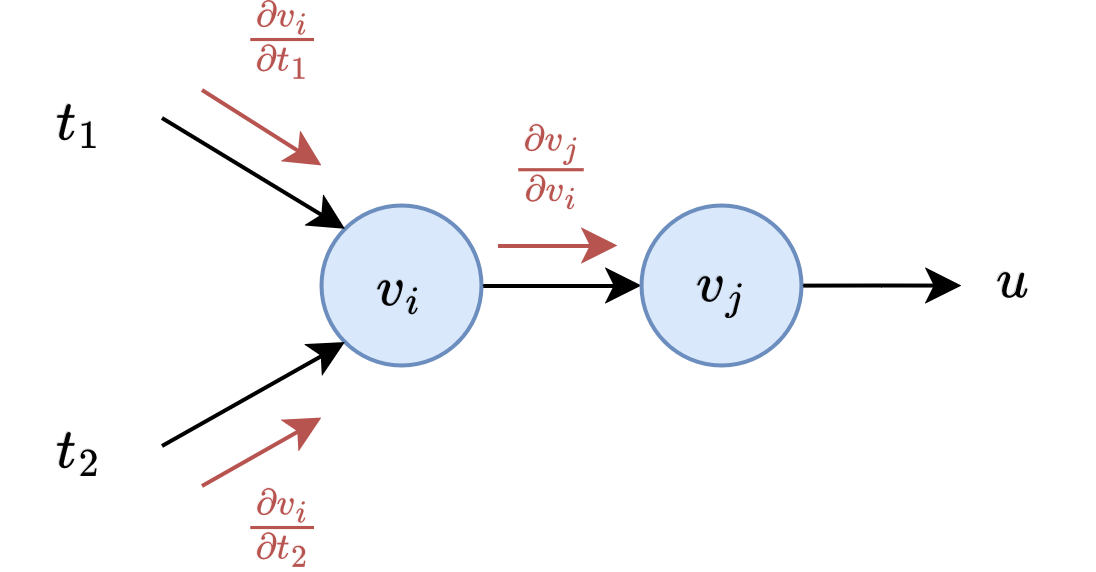
\includegraphics[width=1\linewidth]{2_3a_chain_rule_forward}
        \caption{Forward mode}
        \label{fig:3a}
    \end{subfigure}%
    \begin{subfigure}[h]{0.5\linewidth}
        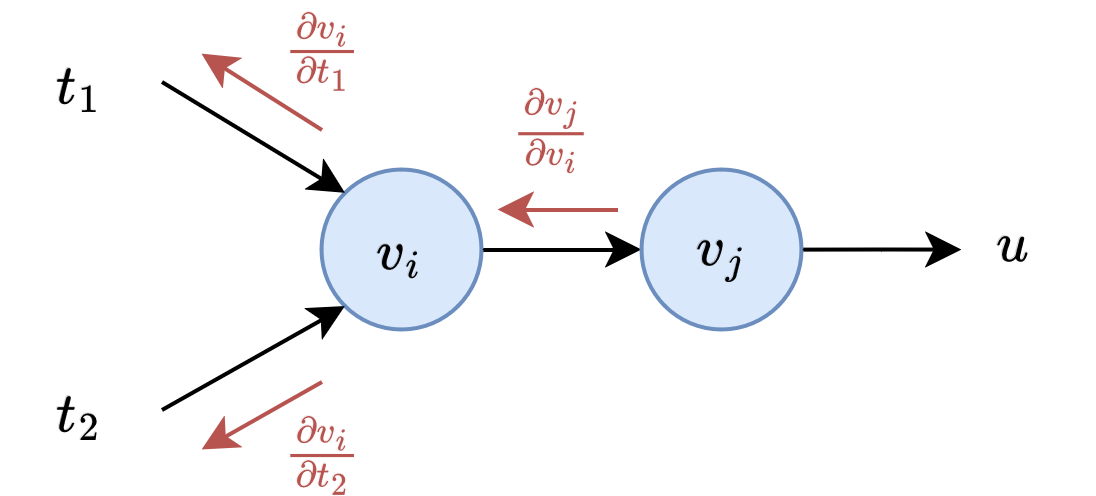
\includegraphics[width=1\linewidth]{2_3b_chain_rule_backward}
        \caption{Backward mode}
        \label{fig:3b}
    \end{subfigure}
    \caption[Chain Rule Forward-Backward Graph]{
        Graphically, interpreting the chain rule in forward mode involves
        propagating gradients from inputs to outputs. Subfigure~\ref{fig:3a}
        visually illustrates this process, showing how node $v_i$ transmits its
        derivative to the subsequent node $v_j$. Conversely, the backward mode
        entails the propagation of gradients from outputs back to inputs, as
        depicted in subfigure~\ref{fig:3b}. This graphical interpretation also
        clarifies how the automatic differentiation (AD) algorithm functions:
        to compute the derivative of a variable $u$ with respect to another
        variable $t$, it simply involves multiplying the gradients that appear
        along the path from $u$ to $t$.
    }
\end{figure*}

Upon completing the backward mode of automatic differentiation, the adjoints of
the input variables are determined. These adjoints represent the partial
derivatives of $y$ with respect to the input variables. This aspect underscores
the efficiency of the reverse method: a single application of reverse mode
yields the gradients for all input variables. With only two traversals of the
computation graph (one forward and one backward) the method achieves a
computational complexity of $O(2n)$. This efficiency makes it particularly
suitable for computing the gradients of loss functions with respect to the
parameters in deep neural networks\sidenote{In the context of deep learning,
reverse mode automatic differentiation is commonly referred to as
\emph{backpropagation}.}, a crucial step in gradient-based optimization. Today,
reverse mode automatic differentiation is the de facto standard for computing
derivatives in the field. Common deep learning frameworks (or AD engines) such
as PyTorch \sidecite{paszke_2017} and TensorFlow \sidecite{abadi_2016}
internally represent computations as graphs and apply reverse mode automatic
differentiation to compute the derivatives on these graphs.

Reverse mode automatic differentiation (AD) is highly efficient for computing
gradients, but it does have a drawback concerning memory efficiency. Since the
values of each intermediate step need to be available before initiating the
backward pass, the entire evaluation trace must be stored in memory. This
requirement can become unfeasible, particularly when dealing with large
datasets or deep neural network models that involve extensive computational
graphs. Such memory demands can limit the scalability of reverse mode AD in
resource-constrained environments or when training extremely large models.
\subsection{Stochastic Gradient Descent}
As previously mentioned, gradient-based optimization methods compute the
gradient of the expected loss with respect to the model's parameters. By
examining the update rule in~\refeq{2_3}, it is evident that the
gradient computation of the expected loss can become problematic. This is due
to the fact that, as the dataset size increases, memory and computational
requirements for reverse mode automatic differentiation to compute the gradient
would escalate significantly, rendering the method impractical for extremely
large datasets. In practical applications, a variant of gradient descent known
as Stochastic Gradient Descent (SGD) is commonly used. The fundamental concept
of SGD involves sampling a subset $\mathcal{B}_r \subset \mathcal{D}_n$ (where
$r \ll n$) at each iteration $t$. Utilizing this subset allows for the
computation of an approximated version of the true expected loss, as
demonstrated in~\refeq{2_12}.
\begin{equation}
    \labeq{2_12}
    \frac{1}{r} \sum_{(x_i, y_i) \in \mathcal{B}_r} L(y_i, f(x_i; \theta)) \approx 
    \frac{1}{n} \sum_{(x_i, y_i) \in \mathcal{D}_n} L(y_i, f(x_i; \theta)) 
\end{equation}
If the samples of the minibatch are independent and identically distributed
from the dataset, the left-hand side of~\refeq{2_12} constitutes a
Monte Carlo approximation of the full loss, and the same principle also applies
to its gradient. The computational complexity of this process grows only with
$r$, which users can directly control\sidenote[][*-12]{In practical terms,
selecting smaller minibatch sizes ($r$) leads to more computationally efficient
iterations but introduces higher variance in the gradient estimates. Conversely,
larger $r$ values produce more accurate gradient estimations but result in less
efficient iterations. This trade-off between efficiency and accuracy must be
carefully managed to optimize the learning process.}.

\section{Neural Networks}
Now that the foundational knowledge on how to train deep learning models has
been established, the focus shifts to the models themselves. Previously, the
model was defined as a plain function to abstract away the real components and
inner workings, which will be discussed extensively in this section. Neural
networks vary from simple to highly complex architectures, each possessing
distinct capabilities and applications. However, all of these architectures are
constructed with high-level differentiable components, such as neurons and
layers\sidenote{To draw a parallel with conventional programming, these
components can be seen as the basic constructs of differentiable programming.}.

\subsection{Perceptron}
The Perceptron \sidecite{rosenblatt_1958} represents one of the earliest models
in the field of artificial neural networks, and serves as the basic building
block the complex models that can be found today. The perceptron draws
inspiration by the biological neuron, which, in a simplified view, functions by
receiving a series of electrical input signals (coming from other neurons) that
are collectively processed\sidenote{Synaptic strengths, or synaptic weights,
determine the influence of one neuron's signal on another.}. These synaptic
weights can change through a process called synaptic plasticity, which is
crucial for learning and memory.
The perceptron mimics this mechanism with these main components:
\begin{itemize}
    \item \textbf{Input nodes}: a vector $\mathbf{x}$ whose the single entry
    $x_i$ represents the signal strength coming from the $i^{th}$ input.
    \item \textbf{Weights}: a vector $\mathbf{w}$ that determines the synaptic
    strength of each input.
    \item \textbf{Bias}: a real value $b$ that can be likened to the neuron's
    resting membrane potential\sidenote{The resting membrane potential is the
    baseline level of electrical charge inside the neuron relative to the
    outside.}.
    \item \textbf{Activation function}: a real valued function $\sigma:
    \mathbb{R} \to \mathbb{R}$ that determines whether the perceptron will
    activate or not based on its activation field\sidenote{The activation field
    of a perceptron is the weighted sum of the inputs plus the bias}.
\end{itemize}
\refeq{2_13} shows the output of the perceptron model, utilizing all the
previously discussed components. Note that the function is parameterized by the
vector of weights and the bias. Consequently, the optimization process will
adjust these parameters to enable the model to learn effectively.
\begin{equation}
    \labeq{2_13}
    \begin{split}
    f(\mathbf{x}; \mathbf{w}, b) &= \sigma \left( b + \sum_{i} \mathbf{w}_i \cdot \mathbf{x}_i \right)\\
    &= \sigma (b + \mathbf{w} \cdot \mathbf{x})
    \end{split}
\end{equation}
Frequently, another formulation for the perceptron model is preferred, where the
bias term $b$ is \emph{"absorbed"} into the weight vector $\mathbf{w}$ by
setting the first weight variable $\mathbf{w}_0 = b$ and fixing the first input
entry to always be $x_0 = 1$. The resulting formulation in~\refeq{2_14}
is equivalent to that in~\refeq{2_13}, offering a more compact notation that
simplifies readability.
\begin{equation}
    \labeq{2_14}
    \begin{split}
    f(\mathbf{x}; \mathbf{w}) &= \sigma \left( \sum_{i} \mathbf{w}_i \cdot \mathbf{x}_i \right)\\
    \end{split}
\end{equation}
The perceptron model is particularly adept at solving linear classification
problems by identifying a hyperplane that separates data points into two
distinct classes within a multidimensional space. It excels in scenarios where
the classes can be divided by a straight line in two dimensions, a plane in
three dimensions, or a hyperplane in higher dimensions. If such a hyperplane
exists, the perceptron model will eventually converge to a solution that
accurately classifies all the training examples.
\begin{marginfigure}[*-8]
  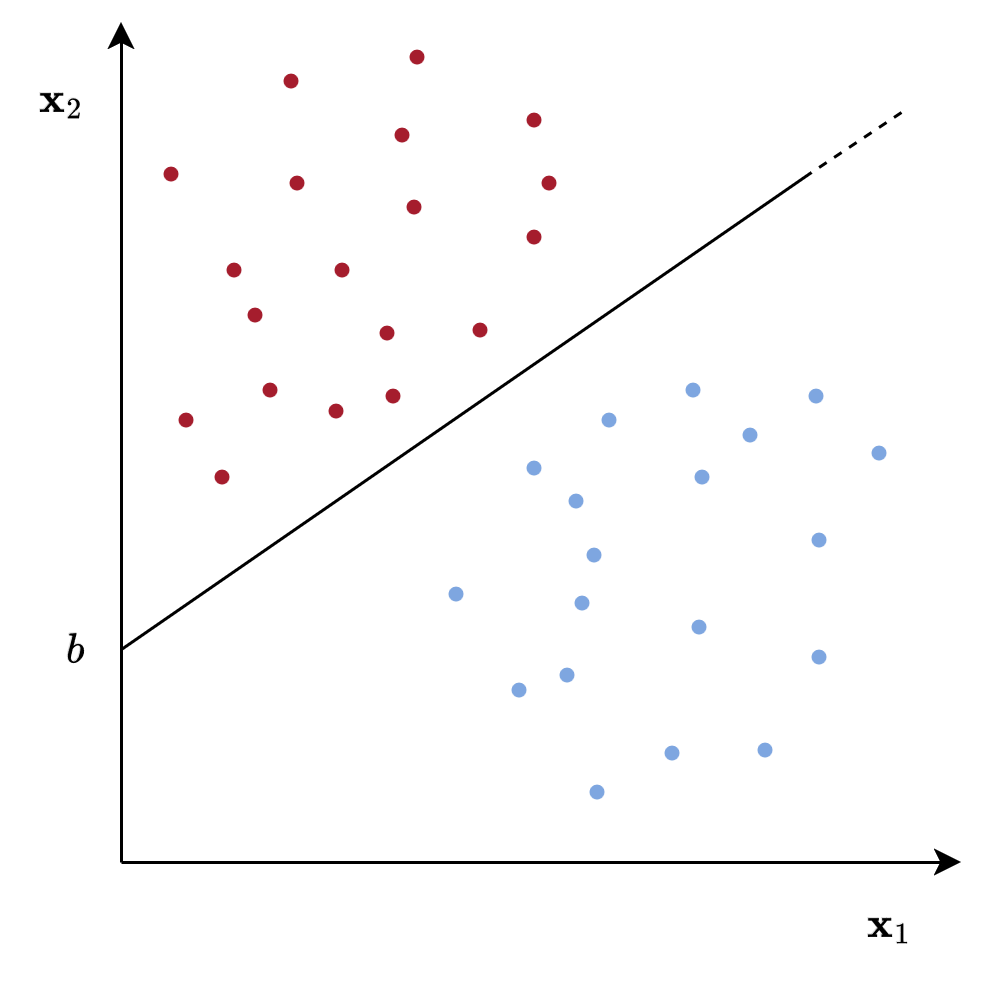
\includegraphics{2_4_linearly_separable}
  \labfig{2_4}
  \caption[Linearly Separable Problem]{
  An example of a linearly separable problem. In this case, $\mathbf{x}$ has
  only 2 elements. The perceptron model creates a line (decision boundary) that
  perfectly separates the examples.
  }
\end{marginfigure}
Common examples of linearly separable problems include binary classification
tasks, such as distinguishing between spam and non-spam emails or identifying
positive versus negative sentiment in text. Additionally, the perceptron can
effectively learn certain Boolean functions, like AND and OR, where the output
can be separated linearly based on the inputs.
\begin{figure}[h]
  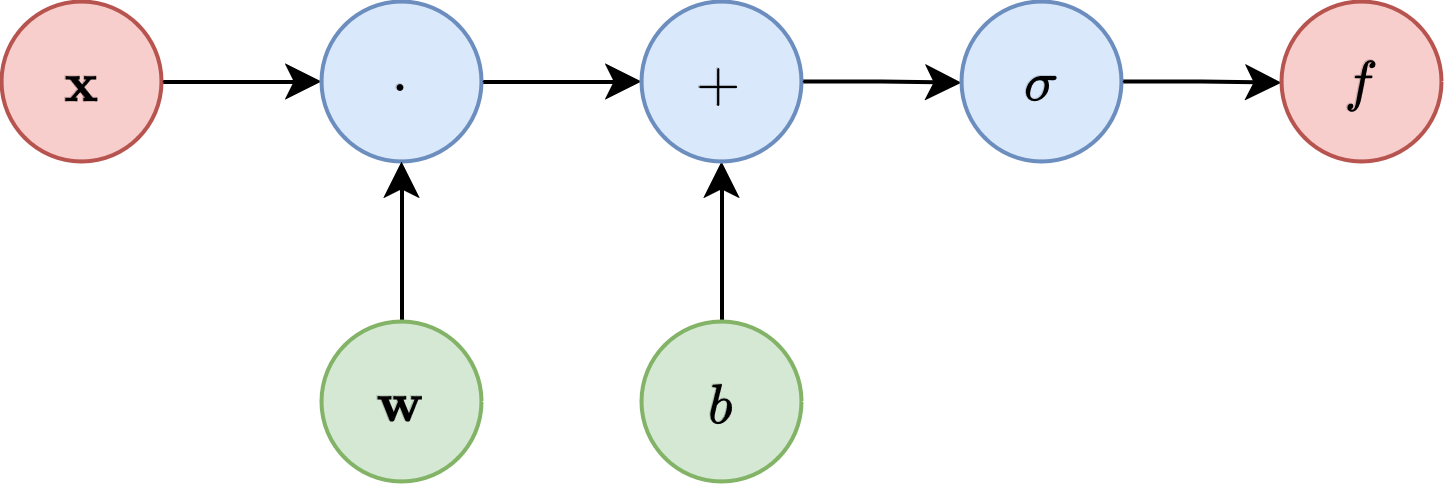
\includegraphics{2_5_perceptron_computational_graph}
  \labfig{2_5}
  \caption[Perceptron Computational Graph]{
      Computational graph of a perceptron. Blue nodes represents
      operators/function, red nodes input/output nodes and green nodes function
      parameters
  }
\end{figure}
Despite its strengths, the perceptron model has notable limitations,
particularly when it comes to handling non-linearly separable problems. In cases
where no single hyperplane can effectively separate the classes, the perceptron
algorithm fails to converge to an accurate solution. A classic example of this
limitation is the XOR problem, where the classes are not linearly separable, and
thus, the perceptron is unable to find a suitable decision boundary. A graphic
example of a non linearly separable problem is depicted in~\reffig{2_6}.
\begin{marginfigure}[*-6]
  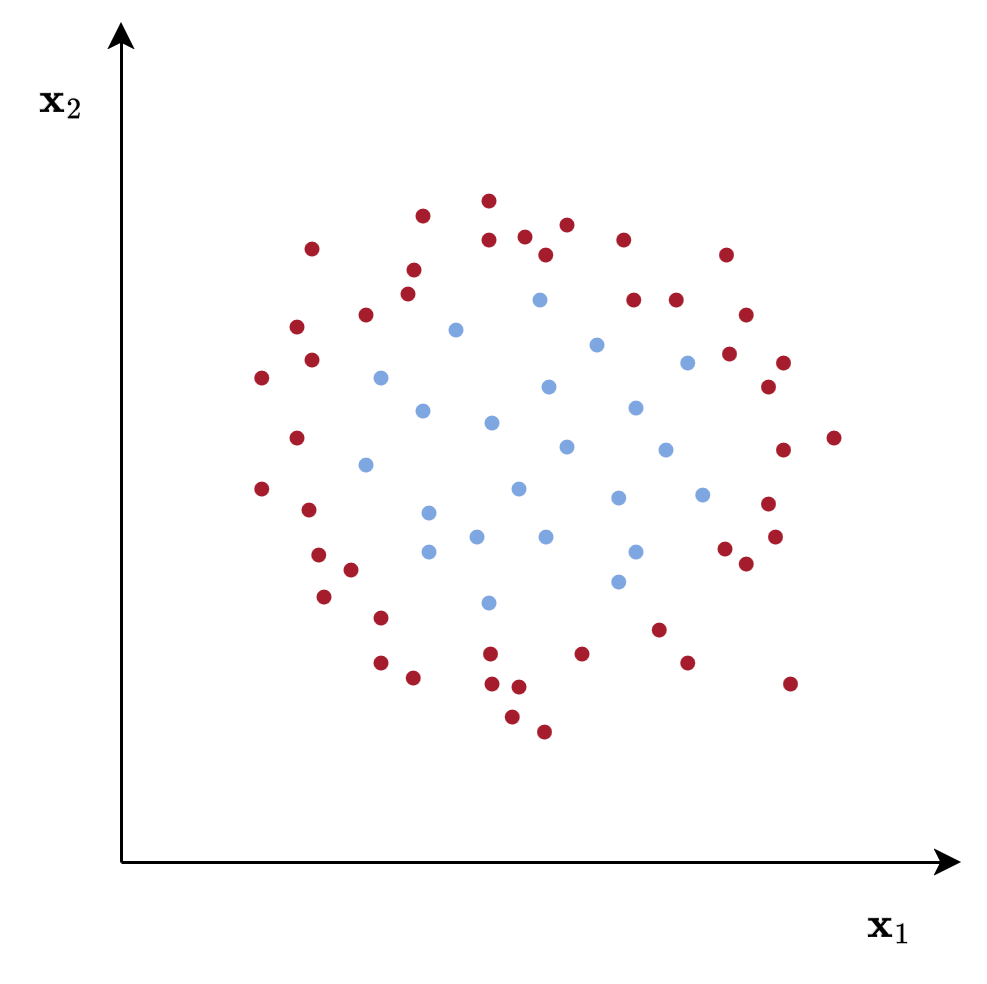
\includegraphics{2_6_non_linearly_separable}
  \caption[Non Linearly Separable Problem]{
  An example of a non linearly separable problem. No line can separate clearly
  the red class from the blue class.
  }
  \labfig{2_6}
\end{marginfigure}
The inability to solve non-linear problems restricts the applicability of the
perceptron model to only a subset of classification tasks, a limitation that
arises from the linear nature of the decision boundary that the perceptron
attempts to establish\sidenote[][*4]{The activation field of a perceptron is in
fact the expression of a line/plane/hyperplane.}.
Many practical problems exhibit non-linear separability, rendering the perceptron
model unsuitable for numerous real-world tasks. Despite the inherent limitations
of the perceptron, it serves as a fundamental building block of neural networks.
By integrating multiple perceptrons, it is possible to construct a fully
connected layer, thereby enhancing the model's capacity to address more complex
tasks.

\subsection{Multi-Layer Perceptron}
Using the perceptron as a foundational element, it is possible to construct a
more sophisticated and general entity: a fully connected layer. A fully
connected layer, also referred to as a network layer, consists of $n$ stacked
perceptrons that share the same inputs. As outlined in~\refeq{2_15}, the
parameters of this layer are encapsulated within a matrix $\mathbf{W} \in
\mathbb{R}^{(n \times m)}$, where $n$ represents the number of perceptrons and
$m$ denotes the number of inputs. Each row of the matrix $\mathbf{W}$ corresponds
to the weight vector $\mathbf{w}$ of an individual perceptron. Furthermore, the
output from this layer is a vector of $n$ elements, with each element reflecting
the output from the corresponding perceptron.
\begin{equation}
  \labeq{2_15}
  F(\mathbf{x}; \mathbf{W}) = (f(\mathbf{x}; \mathbf{W}_1), \dots, f(\mathbf{x}; \mathbf{W}_n))
\end{equation}
Instead of computing the output of each perceptron indipendently, it is possible
to compute the output of all perceptrons of the entire layer in parallel, with
just one matrix-vector multiplication as shown in~\refeq{2_16}.
\begin{equation}
    \labeq{2_16}
    F(\mathbf{x}; \mathbf{W}) = \sigma \left( \mathbf{W} \cdot \mathbf{x} \right )
\end{equation}
By utilizing this new construct, it is possible to develop arbitrarily powerful
models. Each layer, being a function, can be composed with other layers to
facilitate sequential computations. In this manner, the output of one layer
becomes the input for the next layer, akin to function composition. 
\begin{equation}
    \labeq{2_17}
    \mathcal{N}(\mathbf{x}; \theta) = (F_1 \circ \dots \circ F_d)(\mathbf{x})
\end{equation}
\marginnote{All layers between $F_i$ with $i \in 2 \dots d$ are called
\emph{hidden layers}.}
\refeq{2_17} formalizes this concept. The resulting model is a fully connected
multi-layered neural network with $d$ layers. Each fully connected layer $F_i$
is parametrized by a weight matrix $\mathbf{W}_i \in \theta$, where $\theta$
represents the set of all parameters of the model.

The models constructed with this framework are called Multilayer Perceptrons
(MLP) \sidecite{rosenblatt_1959} or Feedfoward Neural Networks (FNN). The main
idea of stacking one layer after another in a feedforward network is to enable
the model to learn a hierarchical mapping of the data. For example, in the XOR
problem, a single-layer perceptron fails because it cannot find a linear
boundary to separate the classes. However, by introducing additional layers,
each layer can learn to transform the input data into a more suitable
representation. The first layer might learn simple features, which are then
combined and transformed by subsequent layers into more complex features. This
hierarchical learning allows the network to create intermediate representations
that progressively disentangle the input data, ultimately enabling the final
layer to classify the data accurately. Thus, the network effectively maps the
original input space into a new space where the classes become linearly
separable.

By mapping inputs into diffeerent high-dimensional spaces, FNNs are able to
learn effectively any non-linear problem. In fact, it has been proven that any
feedforward network composed of two layers can approximate any continuous
function on compact subsets of $\mathbb{R}^n$ to arbitrary accuracy, provided it
has a sufficient number of neurons and the appropriate activation functions
\sidecite{leshno_1993}. Feedforward networks are therefore said to be
\emph{universal approximators}.

\subsection{Convolutional Networks}
While the extreme generality of feedforward models (due to their ability to
approximate any function), makes these models very powerful, it also introduces
an additional problem. To illustrate this, consider that each model
configuration $\theta$ of a feedforward network (FFN) represents a point in the
high-dimensional space of all possible model configurations called the
\emph{hypotheses space}. In this vast configuration space, only a small subspace
is relevant for solving the specific problem at hand (i.e., configurations that
make the model perform the chosen task). However, as the number of parameters in
the network grows, the dimensionality of this space increases, leading to an
exponential explosion of possible configurations for the optimization method to
explore. \marginnote{Another problem also arises from the high time and space
complexity of gradient computations, which grows linearly with the number of
parameters, but the parameters themselves of a feedforward network grow
exponentially as the number of neurons increases.}

To mitigate this issue, FFNs are deliberately made less powerful by encoding
inductive priors into the model. Inductive priors are assumptions about the type
of data the model will process and the tasks it must solve. By incorporating
these priors, the expressive power of the models is effectively constrained,
\emph{limiting} the space of all possible configurations. This confinement helps
gradient-based optimization methods focus on regions containing plausible
solutions to the problem at hand.

Convolutional Neural Networks (CNNs)
\sidecite{lecun_cnn_1989}\cite{fukushima_neocognitron_1980} are a type of neural
network architecture that encode specific inductive priors, facilitating the
processing of image data. These priors are:
\begin{itemize}
    \item \textbf{Locality}: image data consists of pixel values where nearby
    pixels are more related than distant ones\sidenote{For example, in an image
    representing a line, pixels will have similar values along the direction of
    the line.}.
    \item \textbf{Weight Sharing}: neurons in the same layer share weights,
    reducing the total number of parameters required for a layer.
    \item \textbf{Pooling}: high-level features (e.g., objects, lines) in an
    image are meaningful only when interpreted over a sufficiently large patch
    of pixels.
\end{itemize}
To encode the first two priors, CNNs utilize a specific type of
layer\sidenote{Recall that layers in neural networks can be seen as the
constructs of a differentiable programming language.} called the
\emph{Convolutional Layer}, which is the origin of their name.

\subsubsection{Convolutional Layer}
Such layer implements a \emph{convolution}, a mathematical operation that (in
the discrete case) consists on computing the sum of the product between two
functions after one is reflected about the $y$-axis and shifted.
\begin{marginfigure}[*-4]
    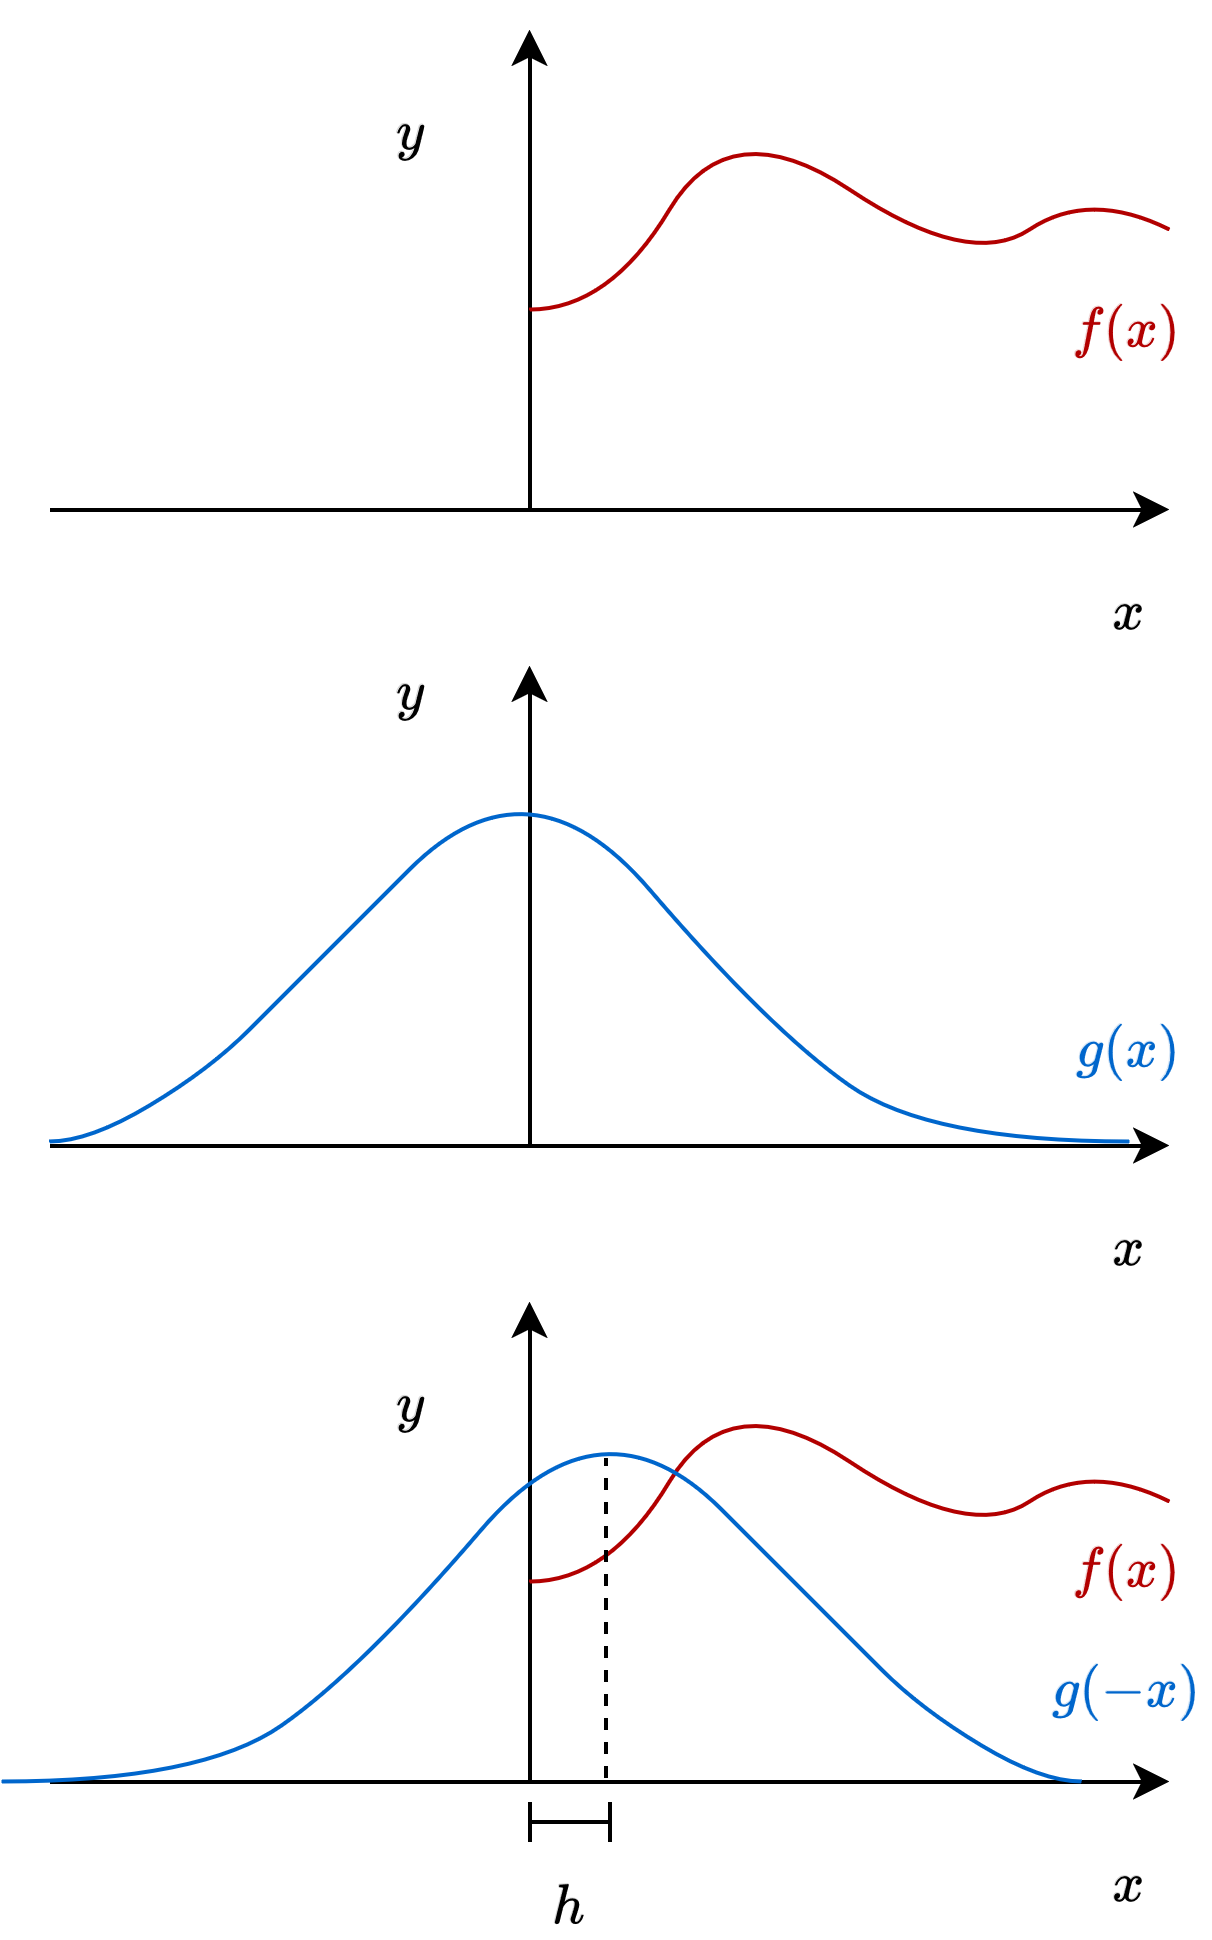
\includegraphics{2_7_convolution_1d}
    \labfig{2_7}
    \caption[Convolution (Mathematical Operation) in 1D]{
    Example of the convolution operation in one dimension. Note that in the
    convolution, $g$ is flipped horizontally ($g(-x)$) and slid over $f$ by a
    displacement $h$.
    }
\end{marginfigure}
From~\refeq{2_18} it can be seen that the convolution actually consists on
computing the similarity between two functions, making one of the function to
progressively slide over the $x$ dimension.
\begin{equation}
    \labeq{2_18}
    (f \star g)(x) = \sum^\infty_{h=-\infty} f(x)g(x - h) 
\end{equation}
The convolution layer implements this operation, where $f$ is the input image
and $g$ (also called the \emph{kernel}) are the learnable parameters (weights)
of the layer. Since images are 2-dimensional bounded discrete
functions\sidenote[][*8]{Images can be seen as the the sampled version of a
2-dimensional real valued signal}, the operation is applied over both
dimensions. \refeq{2_19} shows the output of a single convolutional
neuron. 
\begin{equation}
    \labeq{2_19}
    C(\mathbf{X}; \mathbf{W})_{x, y} = \sum^{M/2}_{m=-M/2}\sum^{N/2}_{n=-N/2}
    \mathbf{X}_{x, y}\mathbf{W}_{(x - m), (y - n)} 
\end{equation}

In~\refeq{2_19}, $M \times N$ represents the dimensions of the
kernel\sidenote[][*4]{Which are typically much smaller than the input image
size.} $\mathbf{W}$ and $\mathbf{X}_{x, y}$ the value of the $(x, y)$ pixel of
the input image. Note that since the input is 2-dimensional, even the neurons
are arranged in a grid-like manner. That is why each neuron's output is
indicized by the variables $x$ and $y$. The results of the convolutional layer
is then also a matrix, called \emph{feature map}. From~\refeq{2_19} it is also
clear how the locality prior is effectively encoded: each neuron process only a
subset of the input\sidenote{That corresponds to a window with dimension $M
\times N$, centered at the $(x, y)$ position.}. The second prior is explained by
the fact that each value of $\mathbf{W}$ is shared between each neuron. That is,
for a single convolutional layer, there exists only an $M \times
N$\sidenote{Without counting other factors such as the sliding window and the
number of channels.} matrix of parameters, which, as previously mentioned, is
much smaller than the input size. The number of parameters of a convolutional
layer is therefore much smaller than its fully connected counterpart.

To be precise, image data is composed of multiple channels which are commonly 3:
red, green and blue. The extension for the convolution layer is straightforward,
it is sufficient to apply the convolution on an additional dimension which
represent the channel, thus, for RGB images, convolutional filters are typically
matrices with dimensions $M \times N \times 3$, where $3$ is the number of
channels.
\begin{marginfigure}
  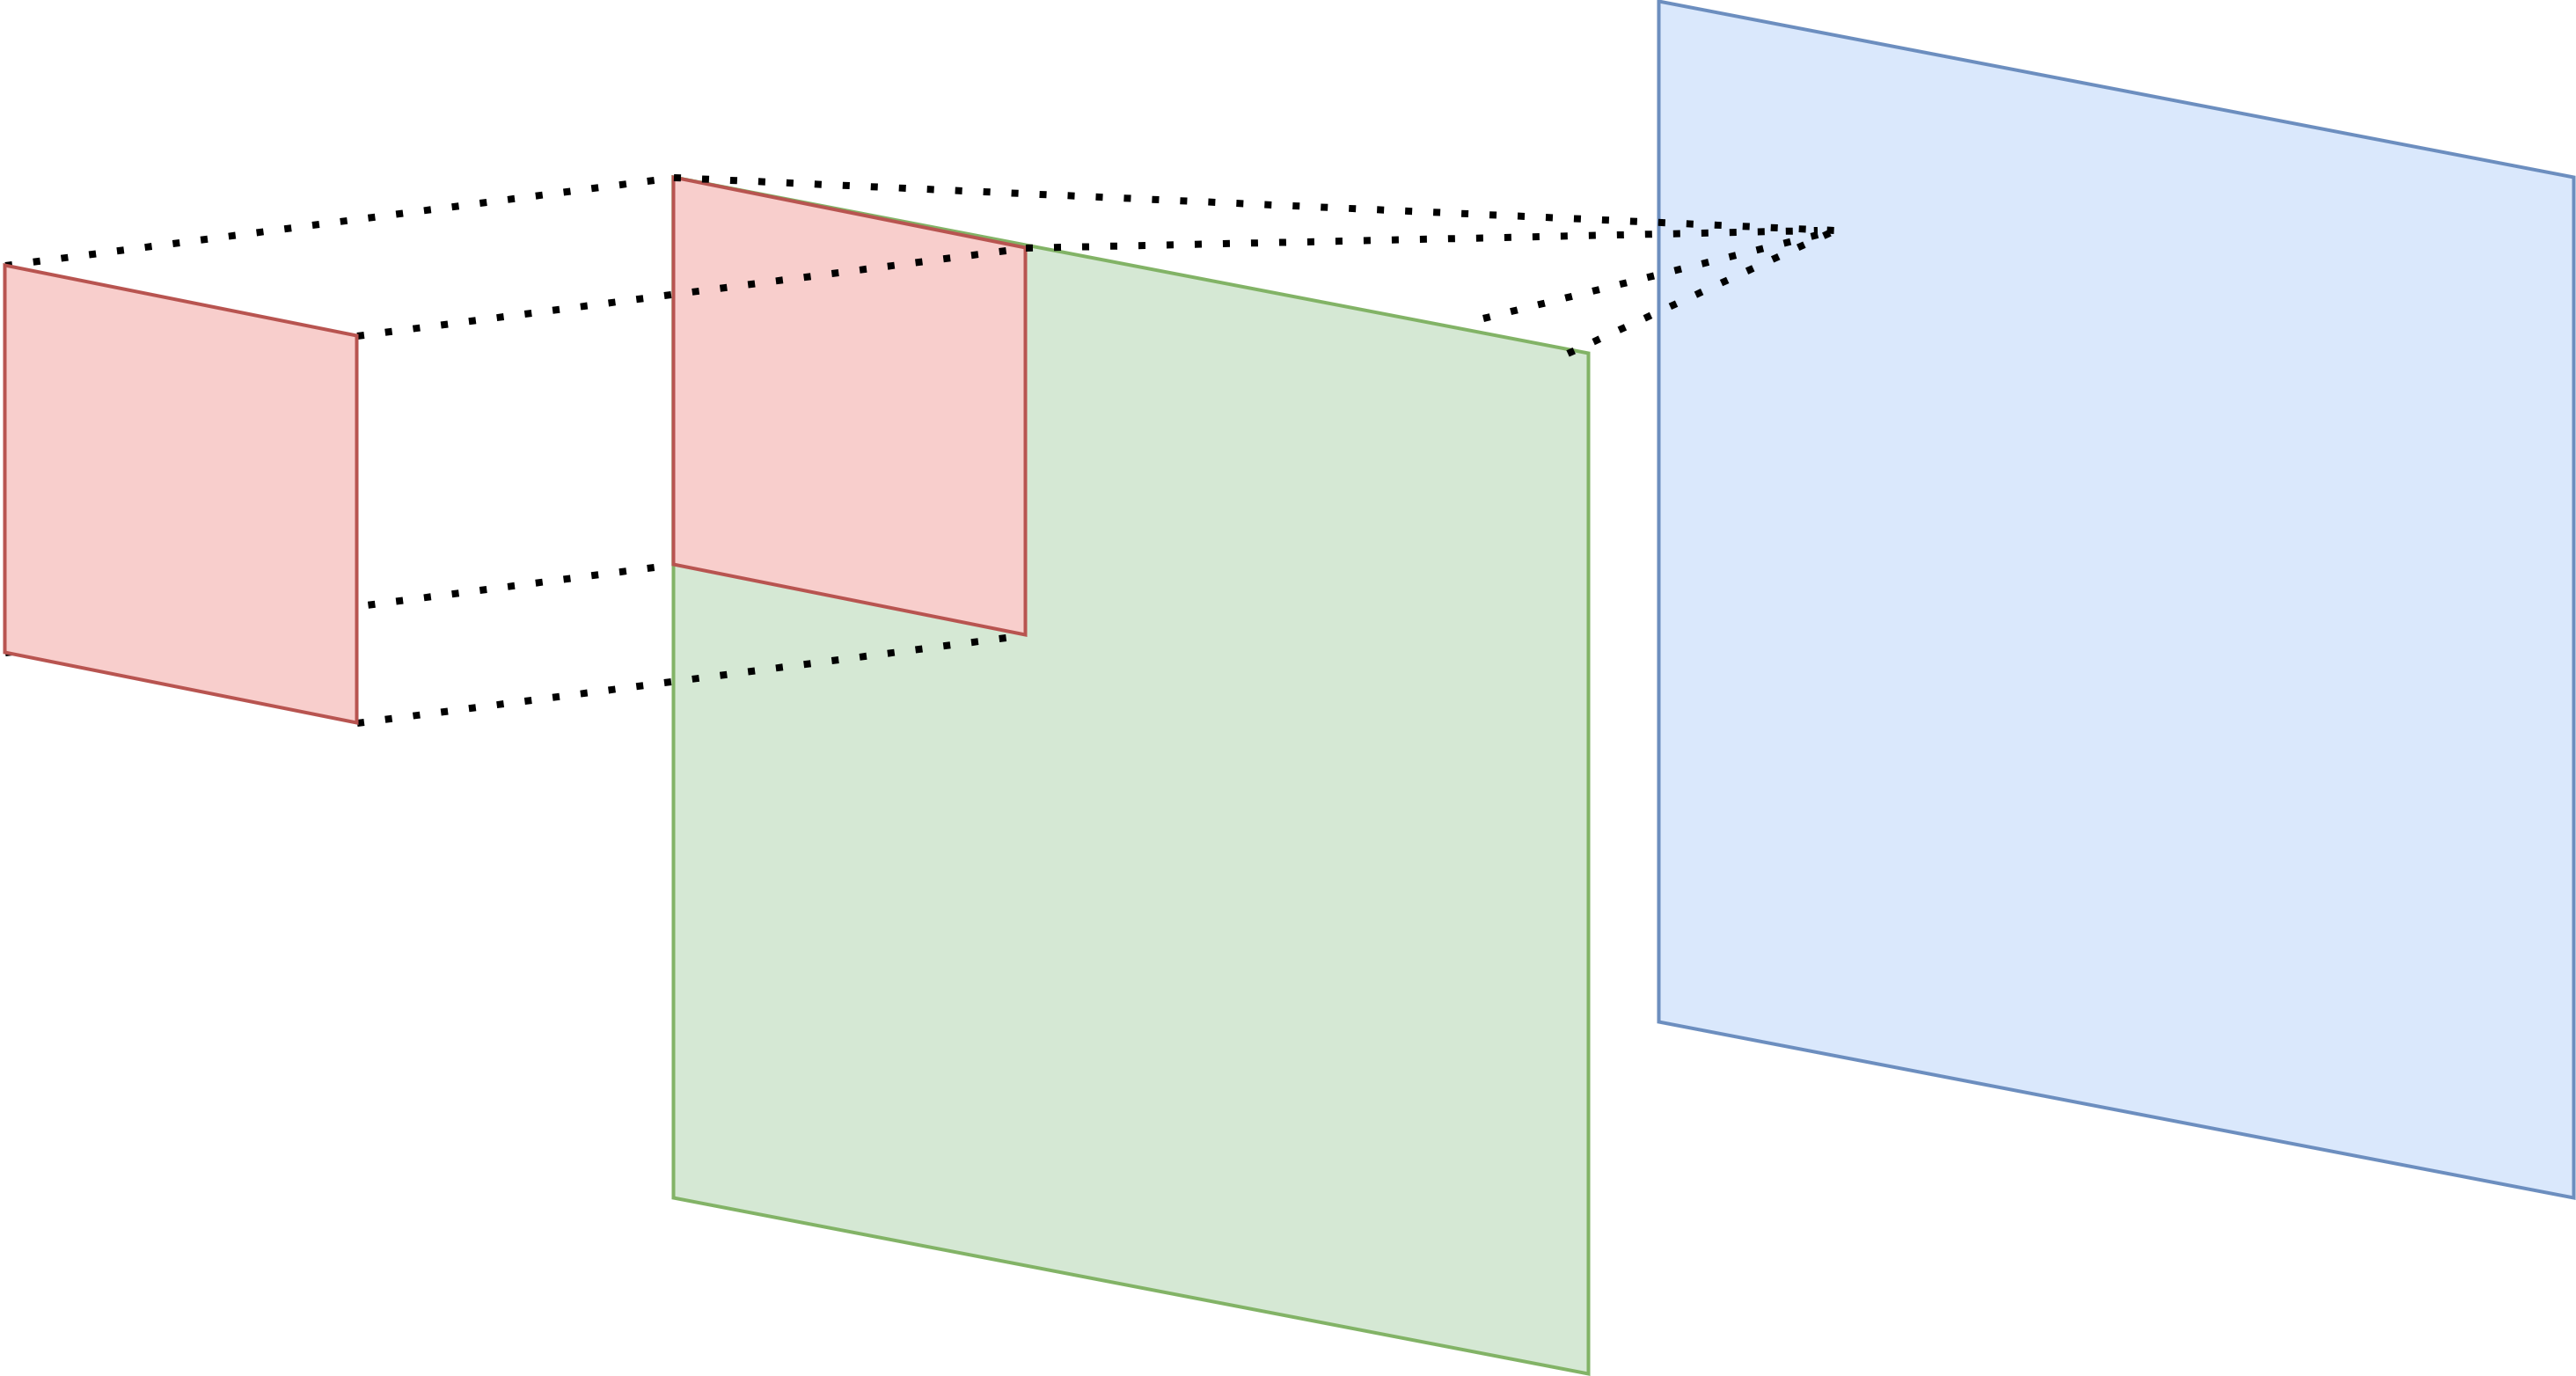
\includegraphics{2_8_convolution_sliding}
  \labfig{2_8}
  \caption[2D Depiction of the Convolution Operation]{
  In the convolution operation the kernel (red square) is applied over the image
  (green square) to produce the corresponding value on the feature map (blue
  square). To compute the next value, the kernel is then slid by a number of positions determined by the \emph{stride}.
  }
\end{marginfigure}
To intuitively comprehend the application of a convolution over a
two-dimensional image, one can visualize it as applying a patch (kernel) of $M
\times N$ elements over the image and computing its weighted sum. This process
involves sliding the patch across all values of the image, with the step size,
known as the \emph{stride}, determining the movement of the kernel to subsequent
positions. In scenarios involving multiple channels, the operation is performed
by applying each patch with identical dimensions to each channel independently
and in parallel. To manage data at the edges of the image, zero padding is
typically applied to the original image, ensuring that the convolution process
can address corner data without loss.

\subsubsection{Pooling Layer}
The pooling prior is encoded by the \emph{pooling layer}. This layer performs a
down-sampling of the input signal, utilizing a sliding window approach similar
to the convolution operation discussed previously. Various down-sampling methods
can be employed, but this discussion focuses on the most commonly implemented
strategies in pooling layers. \refeq{2_20} illustrates the output of an average
pooling neuron and a max-pooling neuron, respectively, applied to an $M \times
N$ window\sidenote{Typical window sizes for pooling layers are $2 \times 2$ and
$3 \times 3$.}.
\begin{equation}
    \labeq{2_20}
    \begin{split}
    P^{avg}(\mathbf{X})_{x, y} &= \frac{1}{L \cdot K} \sum^{L/2}_{l=-L/2}\sum^{K/2}_{k=-K/2} \mathbf{X}_{x - l, y - k}\\
    P^{max}(\mathbf{X})_{x, y} &= \max_{\substack{l \in -L/2, \dots, L/2\\k \in -K/2, \dots, K/2}} \mathbf{X}_{x - l, y - k}
    \end{split}
\end{equation}
Just as the convolution, this process is applied in a sliding window manner. It
follows that the considerations regarding edge handling and striding made
previously are valid for this layer as well. Another important consideration
regarding the pooling layer is that it does not contain any learnable
parameters, which significantly reduces the computational complexity of the
model.

\subsubsection{Network Architecture}
Having discussed the fundamental building blocks of convolutional networks, the
focus now shifts to the actual model architecture, specifically how these blocks
are arranged to construct a model.
Typical convolutional neural network architectures consist of two main
components: a feature extractor and a fully connected head. The feature
extractor comprises a series of convolutional and pooling layers. The rationale
behind this structure is that convolutional layers, through the application of
filters to the input image, generate feature maps that emphasize various image
aspects, such as edges, textures, and complex patterns. Conversely, pooling
layers select the most significant features by down-sampling the input, thereby
reducing the spatial dimensions of the feature maps. The sequential application
of these operations progressively transforms the input data into smaller feature
maps that capture increasingly abstract information about the image\sidenote{
For example, initial convolutional layers might detect simple features such as
edges and corners, while deeper layers might recognize more complex structures
like shapes and objects.}.

The feature extractor is also referred to as the \emph{encoder} because it
encodes the image data into a compact representation containing all the salient
features necessary to solve the task for which the network has been optimized.
Consider, for instance, a CNN that processes input images with three channels
(RGB) and dimensions $W \times H$. Through the progressive application of
convolution and pooling layers, the final feature map (the output of the
encoder) might have dimensions of $8 \times 8$. The output of the model is often
\emph{flattened}, meaning it is reshaped into a one-dimensional vector,
resulting in an output of 64 features. Consequently, the encoder part of the
network can be viewed as a mapping $\mathbb{R}^{W \times H \times 3} \to
\mathbb{R}^{64}$. This 64-dimensional space is called the \emph{latent space}
because the vectors in this space contain \emph{latent} (hidden) features that
the model has learned during training.
\begin{figure}
  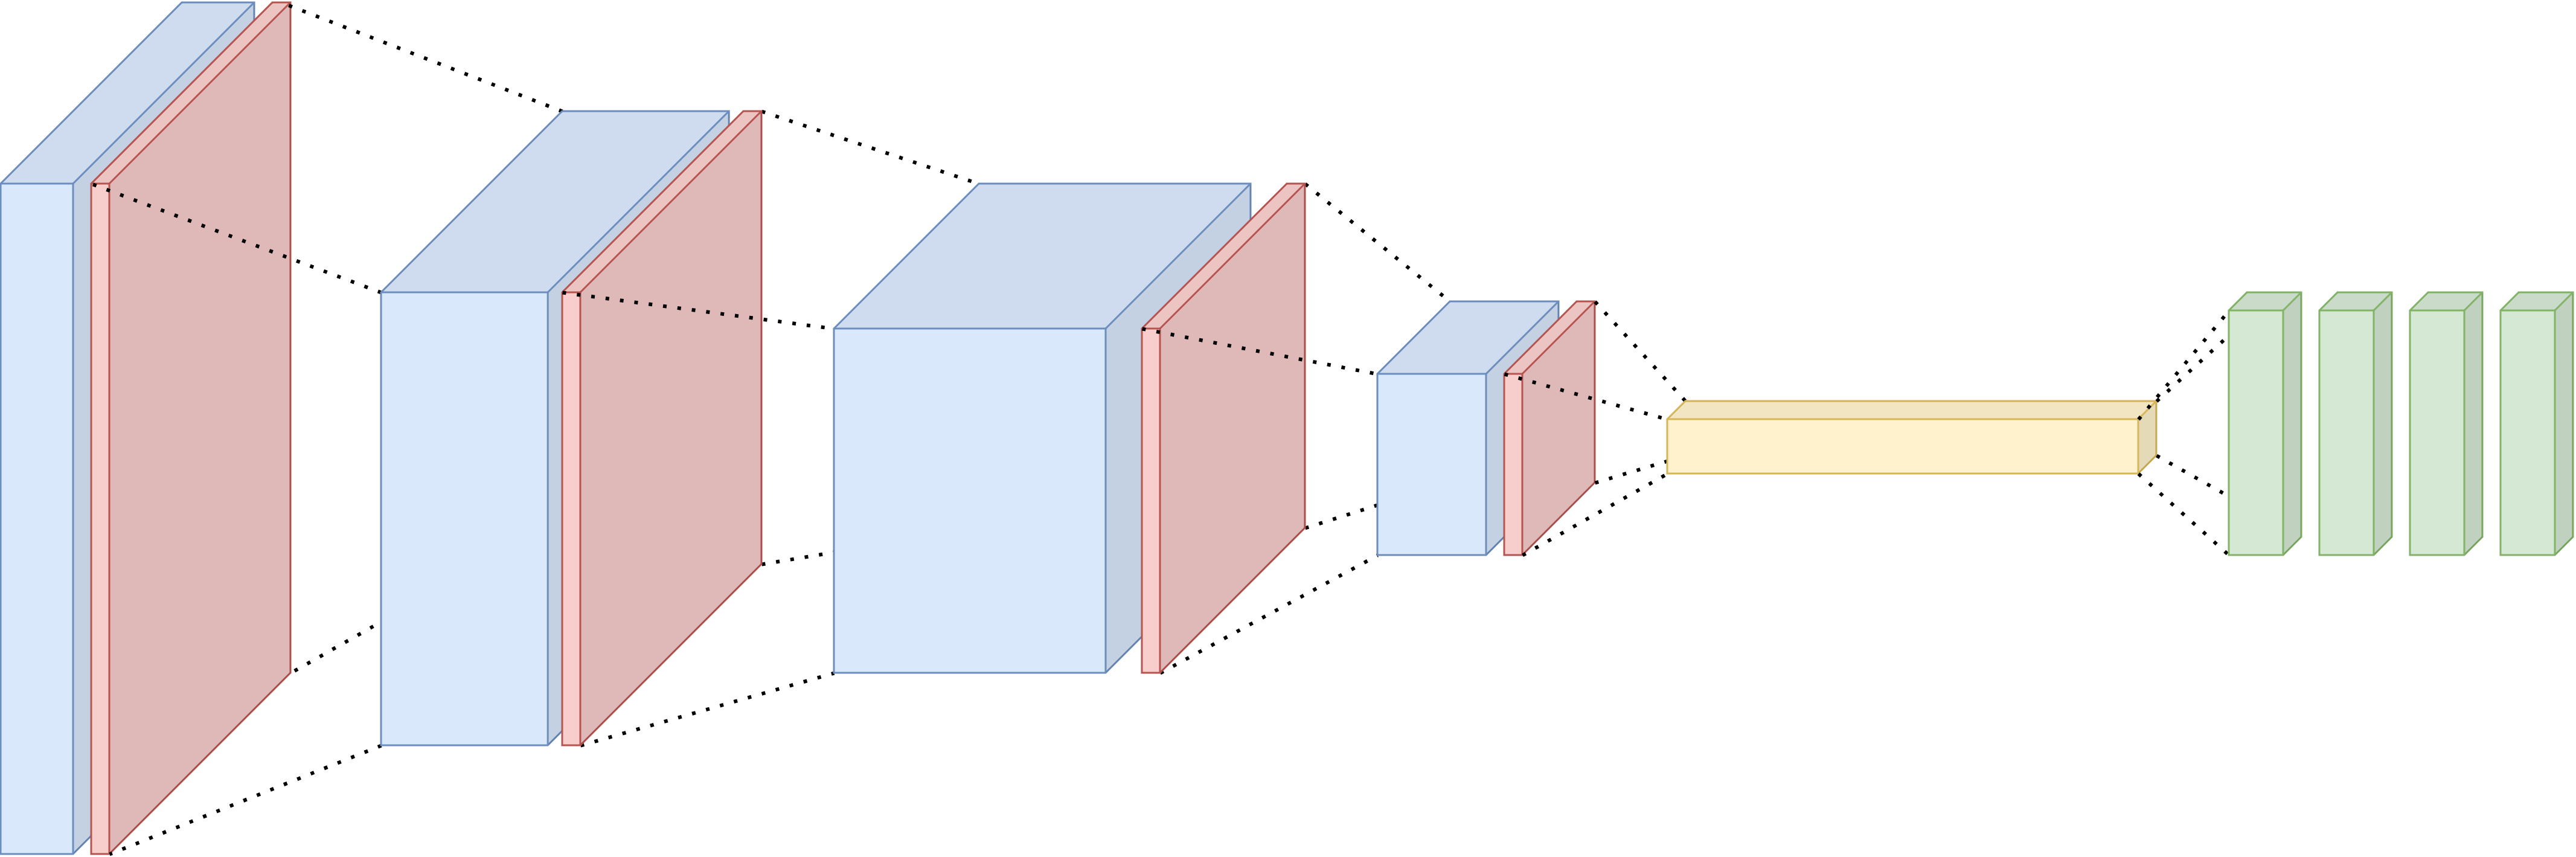
\includegraphics{2_9_convolutional_network}
  \caption[Convolutional Network Architecture]{Graphical depiction of
  Convolutional Neural Network Architecture. In blue are represented
  convolutional layers. Their depth is proportional to the number of filters
  applied in parallel by the layer. In red are depicted the pooling layers,
  while in green the fully connected layers. The yellow block represents the
  hidden representation, that is, the flattened vector that represents the
  encoder's output.}
  \labfig{2_9}
\end{figure}
The encoding part of the model serves to extract all salient features from the
image, progressively selecting them until a compact representation of the input
is obtained. This representation is then fed into the second part of the model:
a fully connected neural network, which performs the actual task, such as image
classification.

Due to the reduced number of parameters in convolutional layers, CNNs can scale
up with a significantly larger number of layers while maintaining manageable
computational complexity. Although all convolutional networks follow a similar
structure, they vary in the number and types of layers, as well as in their
hyper-parameters. Extensive research has been dedicated to identifying the
optimal convolutional network architecture, focusing on the most effective
number and configuration of convolutional, pooling, and fully connected layers.
\reftab{2_3} summarizes some of the most prominent convolutional architectures
found in the literature, along with their total number of parameters.
\begin{margintable} %[ht]
    \resizebox{\textwidth}{!}{
    \begin{tabular}{ l c } \toprule Architecture & Parameters \\ \midrule
        AlexNet \cite{krizhevsky_alexnet_2012} & 60M\\ VGG-16
        \cite{simonyan_vgg_2015} & 138M\\ ResNet18 \cite{he_resnet_2016} &
        11.4M\\
        DenseNet100 \cite{huang_densenet_2018} & 0.8M\\
      \bottomrule
    \end{tabular}
    } 
    \caption[Common Convolutional Network Architectures]{
    Common convolutional network architectures, along with their total number of
    parameters. The architectures are arranged chronologically from older to
    more modern designs. It is noteworthy how the number of parameters has
    decreased over the years, attributed to the development of more efficient
    techniques, which are beyond the scope of this discussion.
    }
    \labtab{2_3}
\end{margintable}
During this work, the ResNet \sidecite{he_resnet_2016} architecture has been
predominantly employed, as will be further discussed in~\refch{anatcl}.
Therefore, it is worth to briefly discus its details here.

\subsubsection{ResNet}
To understand the rationale behind the ResNet architecture, it is crucial to
first comprehend the vanishing gradient problem. As discussed previously,
gradient-based optimization methods function by calculating the gradient of the
loss with respect to the model's parameters. These gradients are computed using
an algorithm that applies the chain rule, multiplying the gradients at each
intermediate computational step. However, a challenge arises when the gradients
from these intermediate steps are small. As these gradients are propagated back
toward the input layers, they can become progressively diminished. This leads to
the vanishing gradient problem, where early layers receive an increasingly
smaller gradient signal, effectively stalling the training of the model as these
layers learn very slowly or not at all. This poses a significant challenge for
the training of deeper networks, as the vanishing gradient problem becomes more
pronounced with an increase in the number of layers\sidenote{This is due to the
proportional increase in the number of dilution steps through which the gradient
must pass.}.
\begin{figure*}
    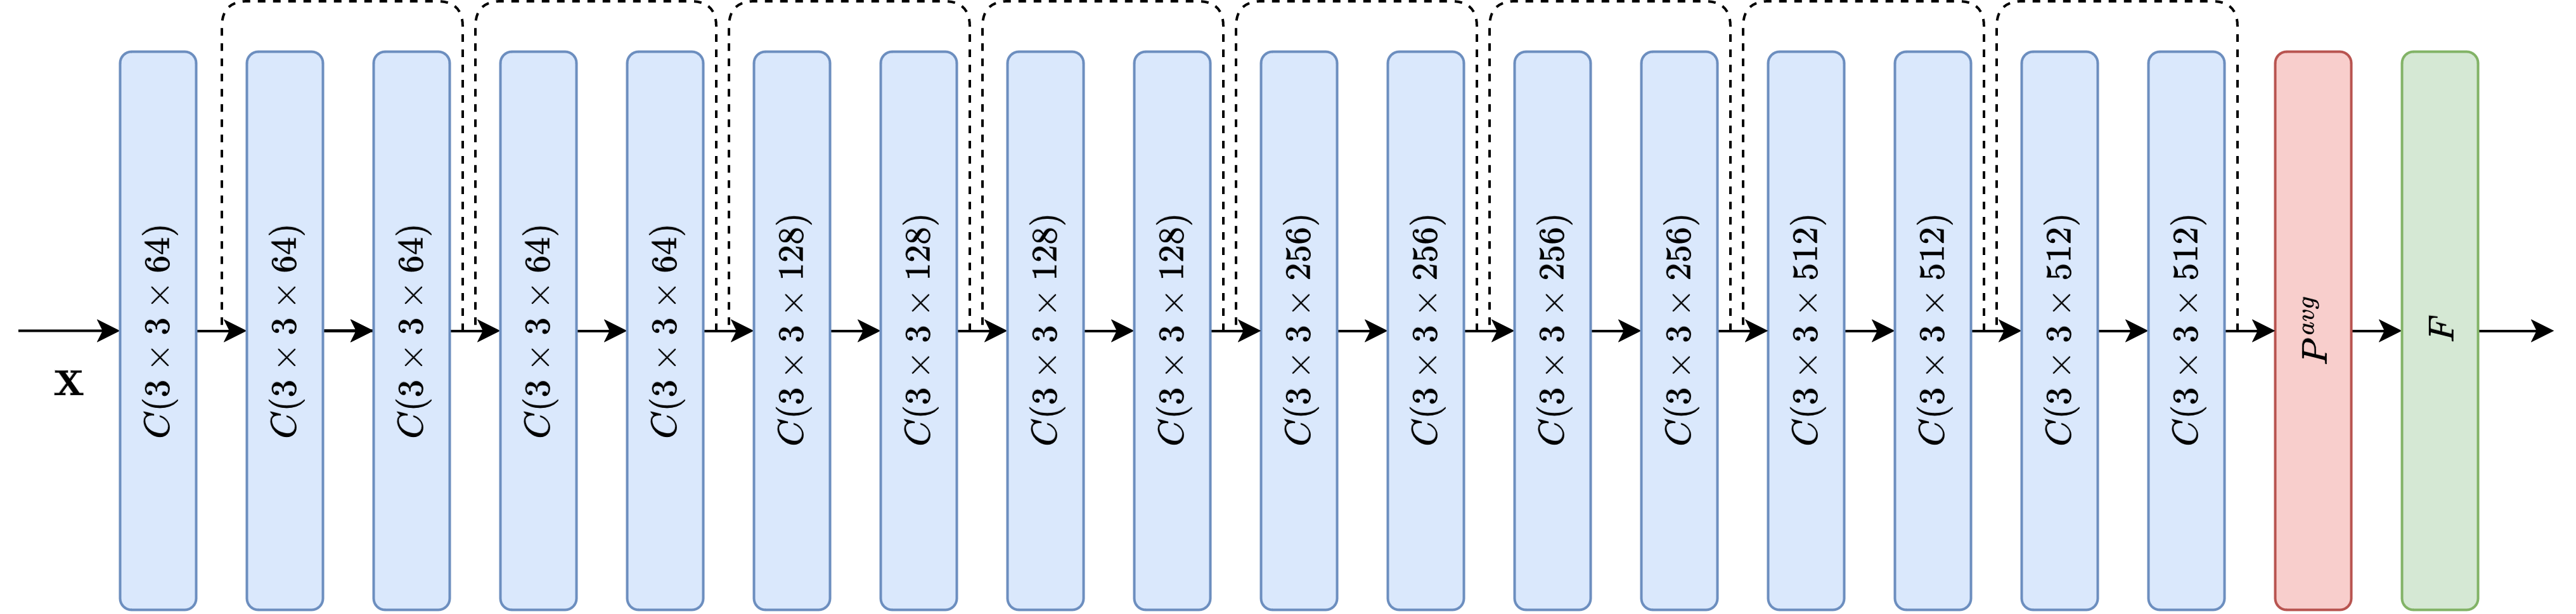
\includegraphics{2_10_resnet_architecture}
    \caption[ResNet-18 Architecture]{Graphical depiction of the ResNet-18
    architecture. The residual connections between layers are depicted in dashed
    lines. Each convolutional block, depicted in blue, is labeled with its
    dimensions $W\times H \times C$, representing width, height, and channel
    count, respectively.}
    \labfig{2_10}
\end{figure*}
However,~\citeauthor{he_resnet_2016}~\cite{he_resnet_2016} demonstrated that
using a special type of connection, known as \emph{residual connections}, can
effectively mitigate this issue. Residual connections allow gradients to flow
directly through the network by skipping layers. By introducing a shortcut path
that bypasses the non-linear transformations, the network can learn identity
functions where necessary, ensuring that the signal is not diluted through deep
layers. This approach has significantly facilitated the training of deeper
networks, as it provides a way for the gradient to pass through without being
dampened by multiple layers of data transformation.
\begin{marginfigure}[*-10]
   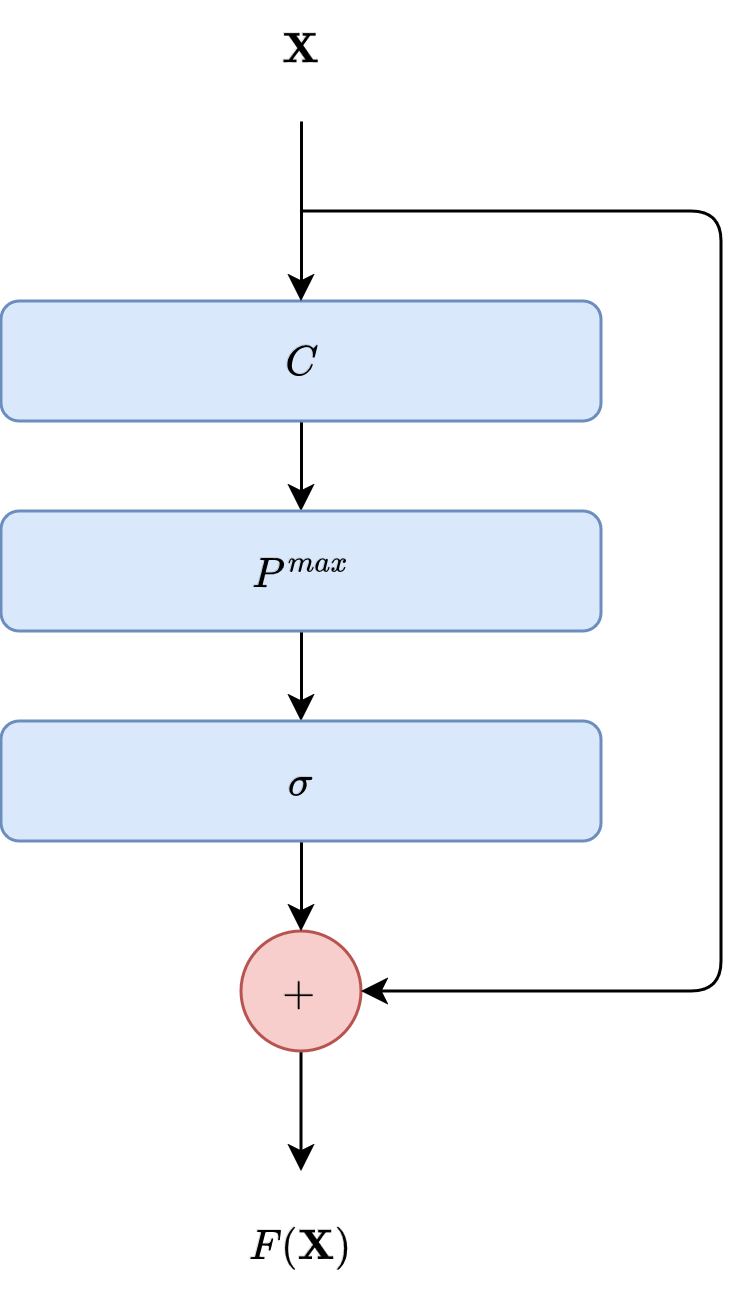
\includegraphics{2_11_residual_block}
   \caption[Residual Block]{A residual block composed of a convolutional layer
   $C$, max pooling layer $P^{max}$ and an activation function $\sigma$. The
   residual connection connects the input $\mathbf{X}$ of the residual block to
   its output $F(\mathbf{X})$ by summing them together. In other words, the
   output of this residual block can be represented as $F(\mathbf{X}) = (C \circ
   P^{max} \circ \sigma)(\mathbf{X}) + \mathbf{X}$.}
\end{marginfigure}
The set of layers that are bypassed by the residual connection is known as a
\emph{residual block}. The skip connection within these blocks is
straightforwardly implemented by summing the input of a residual block to its
output. ResNet incorporates these fundamental units, each comprising
convolutional layers. In the original paper by
\citeauthor{he_resnet_2016}~\cite{he_resnet_2016}, the authors propose different
versions of this architecture, reflecting various sizes and depths. In this
thesis, the primary focus has been on employing the ResNet-18 architecture, a
variant of the ResNet family that consists of 18 layers. This architecture
adheres to the typical design principles of convolutional networks but
incorporates residual connections between layers to enhance learning in deeper
networks. \reffig{2_10} provides a detailed illustration of the ResNet-18
architecture.
